\section{Early Results}\label{sect:results}

This section will demonstrate some of the first results of the CoF and ULFM
work.  Results are from the ``Dancer'' test platform unless noted otherwise.
Dancer is a 16-node cluster where each node consists of two 2.27GHz quad-core
Intel E5520 CPUs, with 20GB/s Infiniband interconnect.

\subsection{Runtime Results}\label{subsect:runtime-results}

\begin{figure}
    \centering
%    \begin{minipage}{.48\linewidth}
        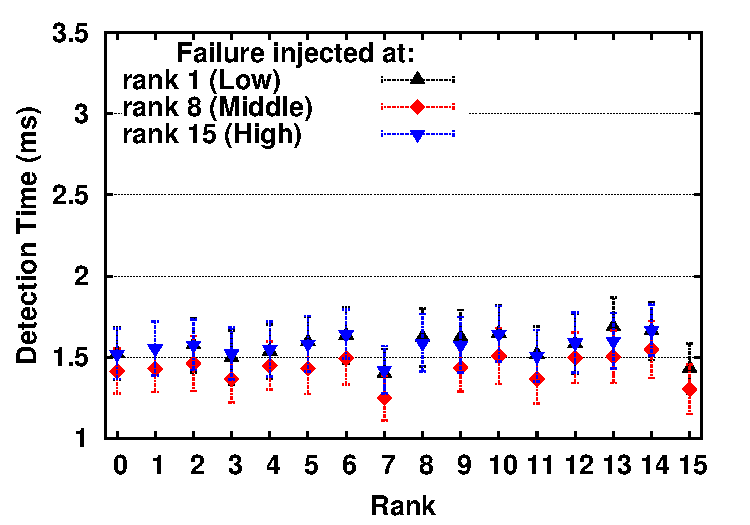
\includegraphics[width=\linewidth]{figures/failure-detection-binomial-errbars}
        \caption{Failure detection time, sorted by process rank, depending on the
        OOB overlay network used for failure propagation.}
        \label{fig:binomial-detection}
%    \end{minipage}
%    \hfill
%    \begin{minipage}{.48\linewidth}
%        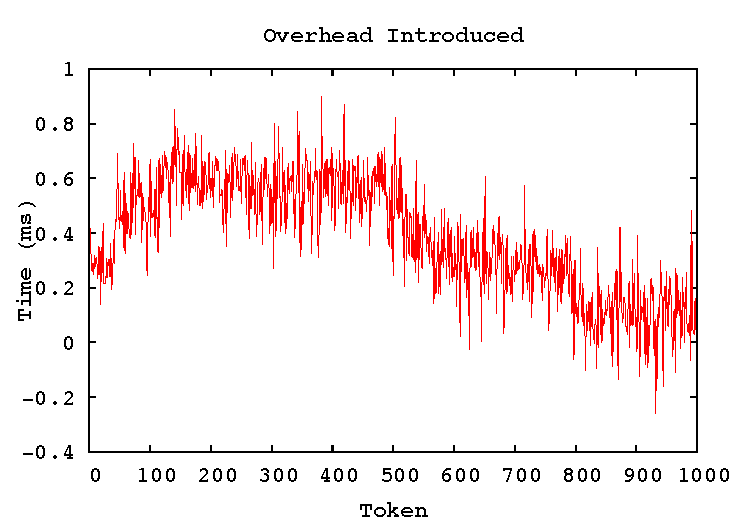
\includegraphics[width=\linewidth]{figures/overhead}
%        \caption{Overhead introduced by resilience changes.}
%        \label{fig:overhead}
%    \end{minipage}
\end{figure}

Our changes to the Open MPI Runtime Environment (ORTE) demonstrate the low
amount of overhead introduced in failure free execution as well as fast failure
detection when failures do occur.

We created a micro-benchmark to measure failure detection time on different MPI
processes. The benchmark uses an \mpifunc{MPI\_BARRIER} to roughly synchronize
the processes, stores the reference start time, then enters a ring algorithm
while injecting a failure at a predetermined location. When the failure is
detected, MPI stores the detection time to determine a relative length for the
failure detection. Figure~\ref{fig:binomial-detection} demonstrates the
detection time for failures in three different locations in the system, ranks 1
(low), 8 (middle), and 15 (high). It demonstrates a binomial OOB topology which
allows for fast, scalable failure detection due to its tree-based topology. The
experiment shows an average of 20 runs with error bars showing the standard
deviation of the runs.

%Using the same micro-benchmark for Figure~\ref{fig:overhead}, we measured the
%overhead introduced by our changes to the Open MPI source by comparing the
%timing results of our resilient code to the Open MPI trunk revision 24614. The
%only change in the benchmark is that failures were not introduced during the
%execution and only the round trip time of the tokens were used. The results show
%that the changes introduced a very small amount of overhead of about 0.5ms. The
%variations in the overhead can be explained by network jitter while the overhead
%mostly comes from small increase in the header size due to data necessary for
%the resilient code.

\subsection{\cof Results}\label{subsect:cof-results}

\begin{figure}
    \centering
%    \begin{minipage}{.48\linewidth}
    \begin{minipage}{.73\linewidth}
        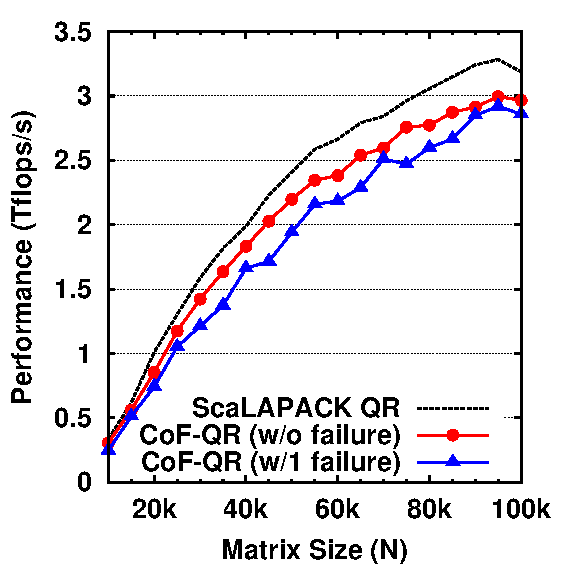
\includegraphics[width=\linewidth]{figures/kraken-new-data}
        \caption{\cof QR on Kraken (Lustre)}
        \label{fig:cof-kraken}
    \end{minipage}
%    \hfill
%    \begin{minipage}{.48\linewidth}
%        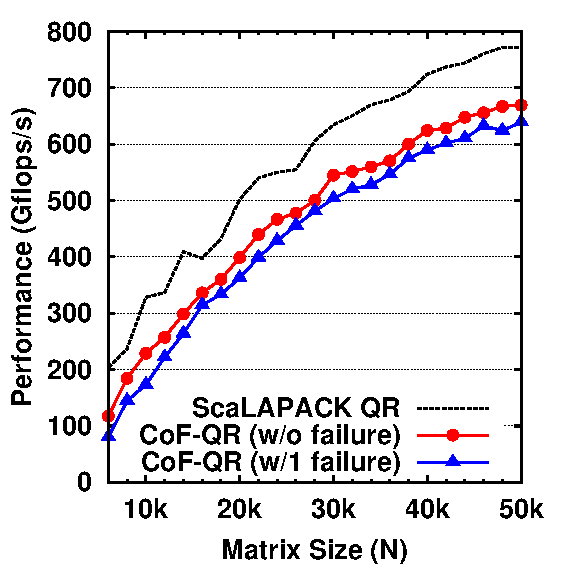
\includegraphics[width=\linewidth]{figures/dancer-performance-data}
%        \caption{\cof QR on Dancer (local SSD)}
%        \label{fig:cof-dancer}
%    \end{minipage}
\end{figure}

To demonstrate the usefulness of the \cof work, Peng Du implemented a \cof
compatible version of a QR factorization. Details of the \cof-QR can be found
in~\cite{Bland:2012tw}. Figure~\ref{fig:cof-kraken} presents the performance of
the \cof-QR code on the Kraken supercomputer. This test was run on a process
grid of 24x24 with a block size of 100. The figure illustrates both the
failure-free and failure-resilient executions compared to the reference
ScaLAPACK implementation.

The result of this experiment demonstrates the feasibility of \cof as a recovery
scheme for some \abft applications. The \cof-QR code was able to achieve
performance results of at least 90\% of the reference ScaLAPACK implementation,
even in the presence of failures, with even better results in the failure-free
case. This shows that compared to a possible performance loss of 25\% or more
with traditional checkpointing, \cof can significantly improve runtime.

\subsection{\ulfm Results}\label{subsect:ulfm-results}

The \ulfm proposal is in its early stages of implementation and testing, however
there have been some comparisons between \ulfm-compatible MPI and 2.2-Standard
MPI to measure the overhead introduced by the new requirements. These tests were
performed on the Smoky system at Oak Ridge National Laboratory. Each node
contains four quad-core 2.0 GHz AMD Opteron processors with 2 GB of memory per
compute core. Nodes are connected with gigabit Ethernet and InfiniBand. Some
shared-memory benchmarks were conducted on Romulus, a $6\times8$ AMD Opteron
6180 SE with 256 GB of memory (32 GB per socket) at the University of Tennessee.
We compare the vanilla version of Open MPI (r26237) with the ULFM enabled
version. 

%Table~\ref{tab:netpipe} demonstrates the low impact on 1-byte latency and
%bandwidth using the NetPIPE benchmark (v3.7). 

Experiments using the NetPIPE benchmark have demonstrated that for all types of
interconnect, the difference between the \ulfm implementation performance and
the vanilla version of Open MPI is negligible. All of the differences are within
the standard deviation of both measurements which shows that any variation is as
likely to be caused by network noise as implementation changes.

%\begin{table*}
%    \begin{center}
%        \begin{tabular}{|l||r|r||r|r||r|}
%            \multicolumn{6}{c}{1-byte Latency (microseconds) (cache hot)} \\
%            \hline
%            \cellcolor[gray]{0.7}\textbf{Interconnect}  & \cellcolor[gray]{0.7}\textbf{Vanilla}   & \cellcolor[gray]{0.7}\textbf{Std. Dev.} &
%            \cellcolor[gray]{0.7}\textbf{\ulfm}         & \cellcolor[gray]{0.7}\textbf{Std. Dev.} & \cellcolor[gray]{0.7}\textbf{Difference} \\
%            \hline
%
%            \cellcolor[gray]{0.9}Shared Memory &  0.8008 & 0.0093 &  0.8016 & 0.0161 &  0.0008 \\
%            \cellcolor[gray]{0.9}TCP           & 10.2564 & 0.0946 & 10.2776 & 0.1065 &  0.0212 \\
%            \cellcolor[gray]{0.9}OpenIB        &  4.9637 & 0.0018 &  4.9650 & 0.0022 &  0.0013 \\
%            \hline
%            \multicolumn{6}{c}{Bandwidth (Mbps) (cache hot)} \\
%            \hline
%            \cellcolor[gray]{0.7}\textbf{Interconnect}  & \cellcolor[gray]{0.7}\textbf{Vanilla}   & \cellcolor[gray]{0.7}\textbf{Std. Dev.} &
%            \cellcolor[gray]{0.7}\textbf{\ulfm}         & \cellcolor[gray]{0.7}\textbf{Std. Dev.} & \cellcolor[gray]{0.7}\textbf{Difference} \\
%            \hline
%            \cellcolor[gray]{0.9}Shared Memory &  10,625.92 &  23.46 &  10,602.68 & 30.73 & -23.24 \\
%            \cellcolor[gray]{0.9}TCP           &   6,311.38 &  14.42 &   6,302.75 & 10.72 &  -8.63 \\
%            \cellcolor[gray]{0.9}OpenIB        &   9,688.85 &   3.29 &   9,689.13 &  3.77 &   0.28 \\
%            \hline
%        \end{tabular}
%    \end{center}
%    \caption{NetPIPE results on Smoky.\label{tab:netpipe}}
%\end{table*}

%\begin{figure}
%    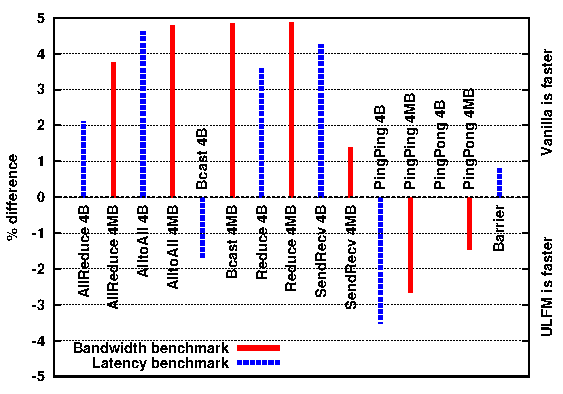
\includegraphics[width=\linewidth]{figures/IMB}
%    \caption{The Intel MPI Benchmarks: relative difference between \ulfm and the
%    vanilla Open MPI on shared memory (Romulus). Standard deviation $\approx$5\%
%    on 1,000 runs.}
%    \label{fig:IMB}
%\end{figure}

%To test the impact on shared memory systems, we used the IMB benchmark suite
%(v3.2.3). Figure~\ref{fig:IMB} shows the duration difference for all the
%benchmarks remains below 5\% in either direction, the standard deviation of the
%implementation on Romulus.

\begin{figure}
    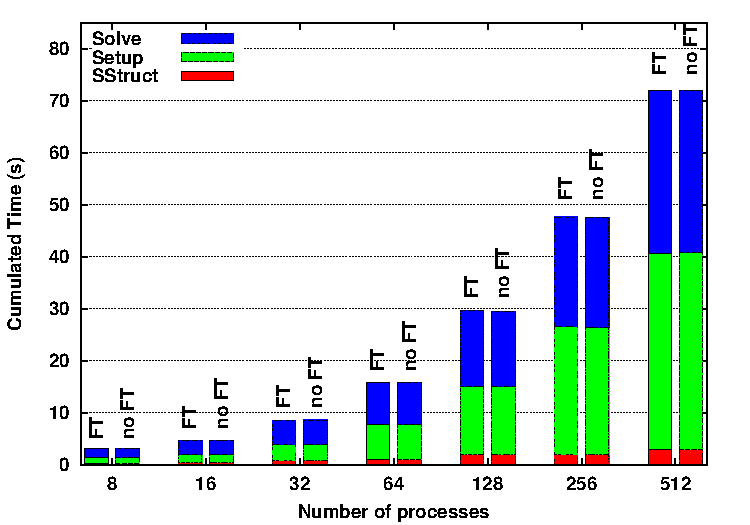
\includegraphics[width=\linewidth]{figures/bargraph.pdf}
    \caption{Comparison of the vanilla and \ulfm versions of Open MPI running
    Sequoia-AMG at different scales (Smoky).}
    \label{fig:sequoia:bargraph}
\end{figure}

To measure the impact of the prototype on a real application, we used the
Sequoia AMG benchmark\footnote{https://asc.llnl.gov/sequoia/benchmarks/\#amg}.
This MPI intensive benchmark is an Algebraic Mult-Grid (AMG) linear system
solver for unstructured mesh physics. A weak scaling study was conducted up to
512 processes following the problem \emph{Set 5}. In
Figure~\ref{fig:sequoia:bargraph}, we compare the time slicing of three main
phases (Solve, Setup, and SStruct) of the benchmark, with, side by side, the
vanilla version of the Open MPI implementation, and the \ulfm enabled one. The
application itself is not fault tolerant and does not use the features proposed
in \ulfm. The goal of this benchmark is to demonstrate that a careful
implementation of the proposed semantic does not impact the performance of the
MPI implementation, and ultimately leaves the behavior and performance of legacy
applications unchanged. The results show that the performance difference is
negligible.

Both of these results are encouraging for future work along the \ulfm path. They
provide proof that an implementation of the new constructs for \ulfm does not
need to cause an increase in overhead generated by the MPI implementation. This
should lead to greater adoption of the \ulfm proposal by multiple MPI
implementations.

%\begin{figure}
%    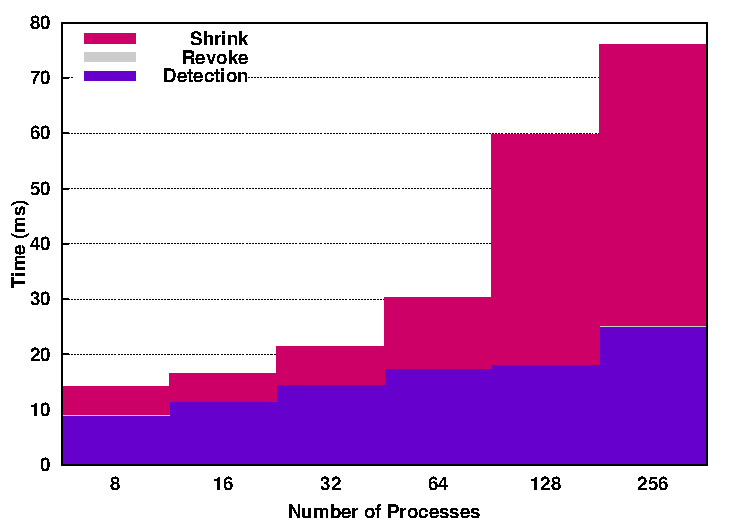
\includegraphics[width=\linewidth]{figures/scalability.pdf}
%    \caption{Evaluation of the Fault Injection Benchmark with full
%    recovery at different scales (Smoky).}
%    \label{fig:frssj:scalability}
%\end{figure}

\begin{comment}

To assess the overheads of recovery constructs, we developed a synthetic
benchmark that mimics the behavior of a typical fixed-size tightly-coupled
fault-tolerant application. Unlike a normal application it performs an infinite
loop, where each iteration contains a failure and the corresponding recovery
procedure. Each iteration consists of 5 phases: in the first phase
(\emph{Detection}), all processes but a designated victim enter a Barrier on the
intracommunicator. The victim dies, and the failure detection mechanism makes
all surviving processes exit the Barrier, some with an error code. In Phase 2
(\emph{Revoke}), the surviving processes that detected a process-failure related
error during the previous phase invoke the new construct
\mpifunc{MPI\_COMM\_REVOKE}. Then they proceed to Phase 3 (\emph{Shrink}) where
the intracommunicator is shrunk using \mpifunc{MPI\_COMM\_SHRINK}. The two other
phases serve to repair a full-size intracommunicator using spawn and
intercommunicator merge operations to allow the benchmark to proceed to the next
round.

In Figure~\ref{fig:frssj:scalability}, we present the timing of each phase,
averaged upon 50 iterations of the benchmark loop, for a varying number of
processes on the Smoky machine. We focus on the three points related to \ulfm:
failure detection, revoke and shrink. The failure detection is mildly impacted
by the scale. In the prototype implementation, the detection happens at two
levels, either in the runtime system or in the MPI library (when it occurs on an
active link).  Between the two detectors, all ranks get notified within 30ms of
the failure (this compares to the 1s timeout at the link level). Although the
revoke call will inject a linear number of messages (at each rank) in the
network to implement the level of reliability required for this operation, the
duration of this call itself is under 50$\mu$s and is not visible in the figure.
The network is disturbed for a longer period, due to the processing of the
messages, but this disturbance will appear in the network only after a failure
occurred.  The last call shown in the figure is the shrink operation. Although
its duration increases linearly with the number of processes (the figure has a
logarithmic scale on the x-axis), this cost must only be paid after a failure,
in order to continue using collective operations. In its current implementation,
shrink requires an agreement, the allocation of a new communicator identifier,
and the creation of the communicator (with \mpifunc{MPI\_COMM\_SPLIT}). Most of
the time spent in the shrink operation is not in the agreement (which scales
logarithmically), but in the underlying implementation of the communicator
creation. 

\end{comment}
